\documentclass[11pt]{article}
\usepackage{hyperref}
\usepackage{graphicx}
\usepackage{float}
\usepackage{geometry}
\usepackage{amsmath,amssymb}
\usepackage{changepage}
\usepackage[labelfont=bf]{caption}
\geometry{
a4paper,
total={170mm,257mm},
left=20mm,
top=20mm,
}
\hypersetup{
    colorlinks=true,
    linkcolor=blue,
    filecolor=magenta,      
    urlcolor=cyan,
}

\title{Analyzing Patterns of Computational Similarity between Protein Kinase Ligands}
\author{Jack Ringer}
\date{July 2025}


\begin{document}

\maketitle


\section{Abstract}
This work investigates whether there is a relationship between the 2D computational similarity of ligands and their activity within specific human protein kinase groups.  
Using data from ChEMBL binding assays, the distribution of pairwise Tanimoto similarity coefficients values computed between all protein kinase ligands was compared against the distribution of pairwise similarity values computed with respect to ligands active within a specific protein kinase group. 
Except for the CK1 group, no significant group-specific differences were found. 
These results suggest there is limited utility of 2D similarity metrics for identifying ligand selectivity across a majority of protein kinase groups. 
However, given the many confounders that exist when performing large scale computational analyses of ChEMBL bioassay data these results are not definitive, and limitations as well as potential follow-ups are discussed in detail. 
All code developed as part of this project can be found on GitHub: \href{https://github.com/Jack-42/ligandActivityAnalysis}{https://github.com/Jack-42/ligandActivityAnalysis}. 

\section{Introduction and Background}
This work explores the relationship between 2D ligand similarity and the activity of these ligands with respect to major protein kinase families, and in particular whether ligands which are active within a particular protein kinase group are more similar to one another than protein kinase ligands generally. 
The following sections provide a brief overview of protein kinases and their classification, molecular similarity, the project's relevance to drug discovery, and related works.


\subsection{Protein Kinases}
Given their (nearly impossible-to-overstate) importance in drug discovery, medicine, and biology + chemistry broadly, an immense amount of effort has been put into classifying proteins. 
One of the most significant protein families studied by drug discovery researchers is the protein kinase family. 
These protein kinases (PKs) are enzymes which modify the function of other proteins via phosphorylation~\cite{lubos_cipak_2022}. 
PKs are involved in many important regulatory roles throughout the cell, and their dysregulation is linked to many types of cancer as well as immune, neurological and infectious diseases~\cite{bhullar_lagaron_mcgowan_parmar_jha_hubbard_rupasinghe_2018}. 
Although all PKs perform phosphorylation, they do not all perform the same function (e.g., some PKs will target different protein domains than others). 

One of the first kinase classifications was published by Manning and other researchers in 2002~\cite{manning_2002}. 
Their research has resulted in the establishment of 8 major groups within the human kinome, which include: AGC, CAMK, CK1, CMGC, STE, TK, TKL, Other, as well as 13 atypical families~\cite{eid_turk_volkamer_rippmann_fulle_2017}.
Generally speaking, these groups (as well as the families and subfamilies they contain) have been classified based on sequence similarity, evolutionary conservation, and known functions. The exceptions are the ``Atypical'' and ``Other'' groups, which serve to classify proteins that don't fit into the other major groups. 
A phylogenetic tree of the human kinome is shown in Figure~\ref{fig:fam_tree}. % TODO: maybe rephrase here

\begin{figure}[H]
    \centering
    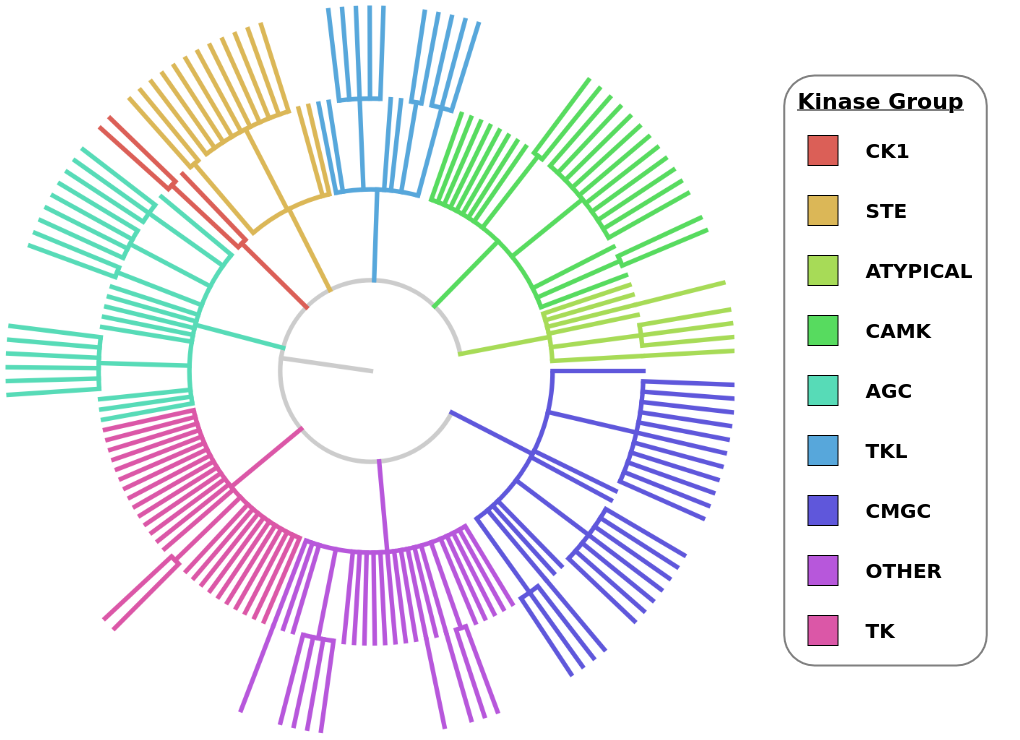
\includegraphics[width=0.7\textwidth]{../figures/protein_family_tree.png}
    \caption{Phylogenetic Tree of the Human Kinome showing major groups as well as families and subfamilies. Generated using ETE4 with data from ChEMBL.}
    \label{fig:fam_tree}
\end{figure}


\subsection{Molecular Similarity}
The similarity property principle (SPP), has been enormously influential in the realm of medicinal chemistry~\cite{maggiora_vogt_stumpfe_bajorath_2013}. 
According to the SPP, structurally-similar compounds often exhibit similar properties. 
Among these properties is biological activity, such that similar compounds often demonstrate similar activity against identical biological targets (i.e., proteins in a majority of cases). 
It is important to note that the definition of “similar” here is ambiguous, and can be measured in a myriad of ways.
Notable excceptions to the SPP are so-called ``activity cliffs'', where a compound which shows high binding affinity (i.e., high activity) against a given target becomes completely ineffective after minor structural modifications~\cite{maggiora_vogt_stumpfe_bajorath_2013,filip_miljkovic_jurgen_bajorath_2018}. 

There are many computational methods for computing molecular similarity between two compounds~\cite{molsim_2024}. Similarity calculations depend both on how compounds are represented (e.g., using molecular graphs, fingerprint vectors, etc) and the particular metric used. 
These similarity metrics typically report a value in the range 0 to 1, with values closer to 1 indicating a higher degree of structural similarity. In addition to computing pairwise similarity, dimensionality-reduction methods (e.g., U-MAP) can be used with clustering algorithms (e.g., K-means) to group together multiple structurally-similar compounds. Other clustering approaches make use of molecular scaffolds or other well-defined structural motifs.

For the purposes of this project, ``similarity'' is determined using Tanimoto coefficients computed from Morgan fingerprints generated by RDKit~\cite{greg_landrum_2024_11396708}. 
The family of Morgan fingerprints (also known as circular fingerprints or extended-connectivity fingerprints) are based upon an algorithm developed by H.L. Morgan~\cite{morgan_1965}. 
The RDKit version of Morgan fingerprints is based upon the implementation described by Rogers and Hahn~\cite{rogers_hahn_2010}. 
Although a detailed description of the Morgan fingerprint is outside the scope of this report, these fingerprints may be summarized as capturing the ``presence of specific circular substructures around each atom in a molecule''~\cite{capecchi_probst_reymond_2020}. 
Morgan fingerprints were chosen because they are widely used within the field of cheminformatics due to (1) the fact that their features are predictive of biological activity and (2) they have proven to be among the best performing fingerprints in virtual screening~\cite{capecchi_probst_reymond_2020}. 

Like Morgan fingerprints, Tanimoto coefficients are widely adopted. 
The Tanimoto coefficient $T(A,B)$ of two bit vectors $A$ and $B$ is computed by the following equation:
\begin{equation}\label{eq:1}
T(A,B) = \frac{|A \cap B|}{|A \cup B|} = \frac{|A \cap B|}{|A| + |B| - |A \cap B|} = \frac{\sum_{i=1}^{n} a_i b_i}{\sum_{i=1}^{n} a_i + \sum_{i=1}^{n} b_i - \sum_{i=1}^{n} a_i b_i}
\end{equation}
\noindent
Tanimoto values range from 0 to 1, with values closer to 1 indicating a higher degree of similarity.
Figure~\ref{fig:ligand_sim} provides a visualization of some pairs of protein kinase ligands identified in this project and their corresponding Tanimoto similarity value.

\begin{figure}[H]
    \centering
    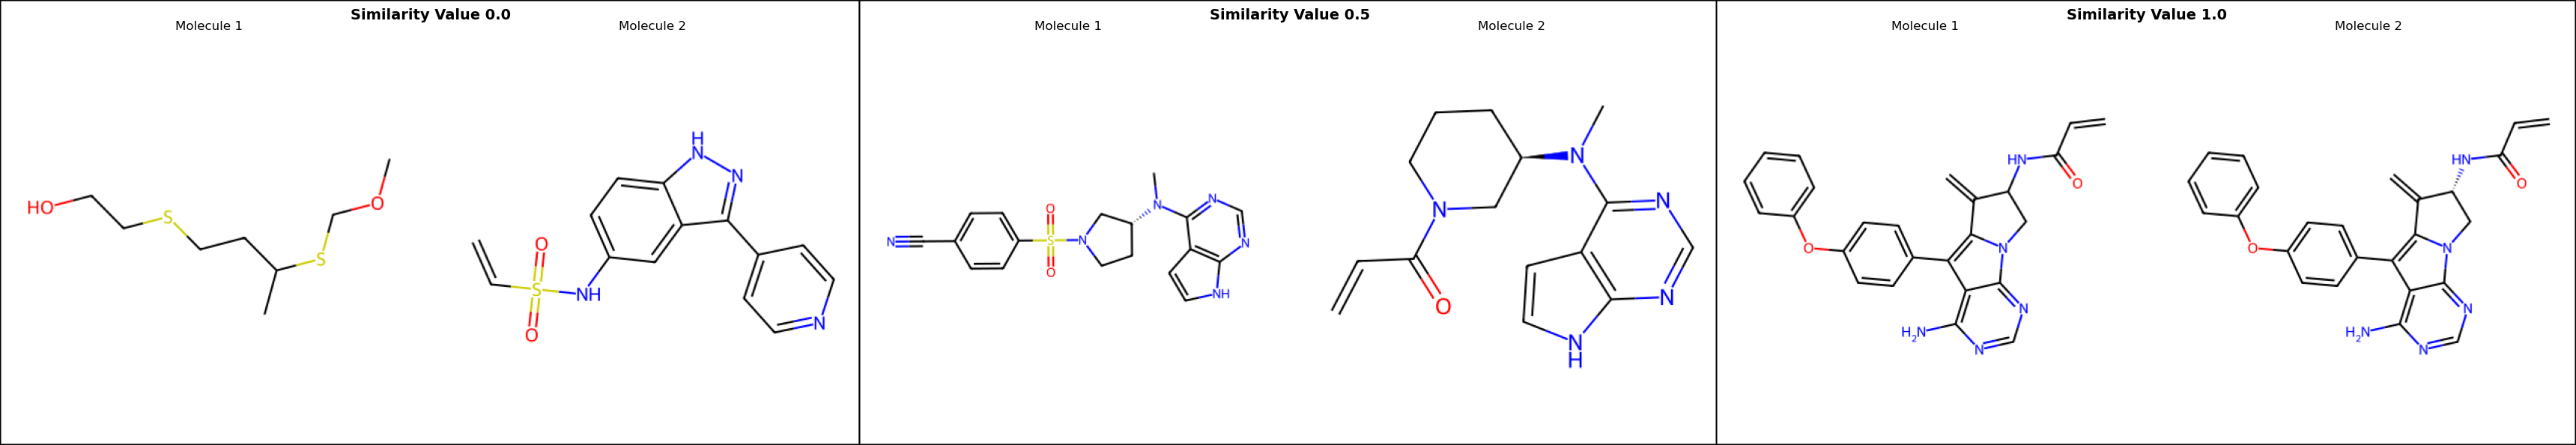
\includegraphics[width=\textwidth]{../figures/ligand_sim.png}
    \caption{Pairs of protein kinase ligands and their Tanimoto similarity values (0, 0.5, 1).}
    \label{fig:ligand_sim}
\end{figure}
 
\subsection{Relevance to Drug Discovery}
% With few exceptions, for a drug to produce an effect it must bind to specific components of cells and tissues~\cite{antolin_ameratunga_banerji_clarke_workman_al-lazikani_2020}. 
% These biological targets are most commonly proteins, although they can also include nucleic acids and peptides~\cite{gashaw_ellinghaus_sommer_asadullah_2011}.  
% A molecule which is ``active'' (as measured by, for example, an IC50 value) against a given disease-related target may be a promising drug candidate. 
% In the case of protein kinases, these drug candidates are often identified from binding assays which measure whether or not the molecules
% TODO: probably need to rephrase above

As mentioned above, protein kinases are involved in a number of human pathologies. 
If there is a relationship between protein kinase group and ligand similarity, then it may be informative to look at the ligands of related kinases (i.e., those belonging to the same group). 
This would be especially beneficial if there are few known ligands for the target of interest, as one could leverage data from well-studied, closely-related proteins to inform the discovery process. 

\subsection{Related Works}
The idea that similar compounds may exhibit similar activities against proteins within the same family (or group) is not new. 
The term ``intrafamily polypharmacology'' (IFP) refers to molecules which have demonstrated activity against multiple proteins belonging to the same family, and has been of special interest in (for instance) studying PARP-1 inhibitors~\cite{passeri_camaioni_liscio_sabbatini_ferri_carotti_giacchè_pellicciari_gioiello_macchiarulo_2015, antolin_ameratunga_banerji_clarke_workman_al-lazikani_2020}. 
Relatedly, previous works have investigated the theory of ``Target-Family-Privileged Substructures'', which suggests that particular chemical substructures are strongly linked to activity against certain protein families~\cite{schnur_hermsmeier_tebben_2006}. 
Several works have developed computational analyses for looking at activity relationships between families~\cite{bajorath_2008}, and works such as \cite{filip_miljkovic_jurgen_bajorath_2018} and \cite{lo_liu_morrissey_kakiuchi-kiyota_johnson_broccatelli_zhong_joshi_altman_2018} have investigated the structures and activities of kinase inhibitors. 


\section{Dataset and Methodology}\label{sec:methodology}
Within this project all data was sourced from ChEMBL (version 35)~\cite{chembl_db_2023}. 
The ChEMBL PostgreSQL database (DB) was downloaded onto a local computer and was then used to carry out data extraction and analysis. 
A Snakemake~\cite{snakemake_2021} workflow was developed to extract relevant assays and ligands (see details below), and additional analyses were performed in Jupyter notebooks. 
As mentioned in the abstract, all code developed as part of this project can be found on GitHub: \href{https://github.com/Jack-42/ligandActivityAnalysis}{https://github.com/Jack-42/ligandActivityAnalysis}. 

The set of active ligands and their relationship to specific human protein kinases was determined using data from single protein target binding assays in the ChEMBL database (version 35)~\cite{chembl_db_2023}. 
In identifying appropriate assays and ligands, the criteria used by Pharos~\cite{pharos_2022} was enforced to ensure that (1) assays were high-quality and (2) a reasonable definition of ``active'' was applied. 
These criteria include the following:
\begin{itemize}
    \item Sample must have a pChEMBL value (i.e., a -Log M value)
    \item Must be from a binding assay
    \item Ligand must have a MOL structure type
    \item Assay must have a target type of SINGLE\_PROTEIN
    \item Sample must have standard\_flag = 1 and exact standard\_relation
    \item Assay must be associated with a journal publication
    \item Sample must have an activity value $\leq \; 30 \text{nM}$
\end{itemize}

In addition to the criteria from Pharos, other filters were also applied based on other prior research and consideration. In particular:
\begin{itemize}
    \item Remove assays where target was a variant/mutant (using implementation described by~\cite{landrum_riniker_2024}).
    \item Filtered out PAINS compounds to remove (some) false positives~\cite{baell_holloway_2010}.
    \item Molecular weight of ligand must fall between [200, 900] Da (this particular range is based upon~\cite{filip_miljkovic_jurgen_bajorath_2018}). 
\end{itemize}

The application of the criteria above to the ChEMBL database (version 35) resulted in a dataset described in Table~\ref{tab:1} below.

\begin{table}[!ht]
\centering
\begin{tabular}{|l|l|}
    \hline
    \textbf{Variable} & \textbf{Value} \\ \hline
    N. Protein Targets & 423 \\ \hline
    N. Assays & 73,487 \\ \hline
    N. Active Samples & 38,622 \\ \hline
    N. Unique Ligands & 9,995 \\ \hline
\end{tabular}
\caption{Counts of proteins, assays, samples, and unique ligands in the dataset}\label{tab:1}
\end{table}

In terms of ligand-target relationships, these were directly inferred from the assays (i.e., if a ligand was present in an active sample in an assay where protein X was specified as the target, then the ligand was considered as active against protein X). 
ChEMBL provides classification information for protein targets, and this information was used to assign ligands to respective kinase group(s) such that a ligand is considered active within a protein kinase group if they were identified as an active within an assay targeting a protein belonging to the group. 
It is perhaps worth noting that, under this definition, a single ligand can belong to more than one kinase group. 
Most commonly this is because the ligand has multitarget activity (i.e., it is active against more than one target, and these targets span more than one group)\footnote{Within the dataset a total of $N=8036 \; (80.6\%)$ of ligands were active against only a single target, $N=1803 \; (18.0\%)$ were active against 2-4 targets, and $N=156 \; (1.6\%)$ were active against $\geq 5$ targets.}. 
However, there are also some rare cases where proteins have been classified into more than a single group by ChEMBL. 
For example, \href{https://www.ebi.ac.uk/chembl/explore/target/CHEMBL3906}{Ribosomal protein S6 kinase alpha 2} belongs to both the AGC and CAMK group according to ChEMBL. 
In these exceptional cases an inclusive approach is taken such that the protein (and any of its active ligands) are considered part of both groups.  
A breakdown of the number of proteins, assays, and ligands belonging to each protein kinase group is provided in Figure~\ref{fig:group_atl_counts}. 


\begin{figure}[H]
    \centering 
    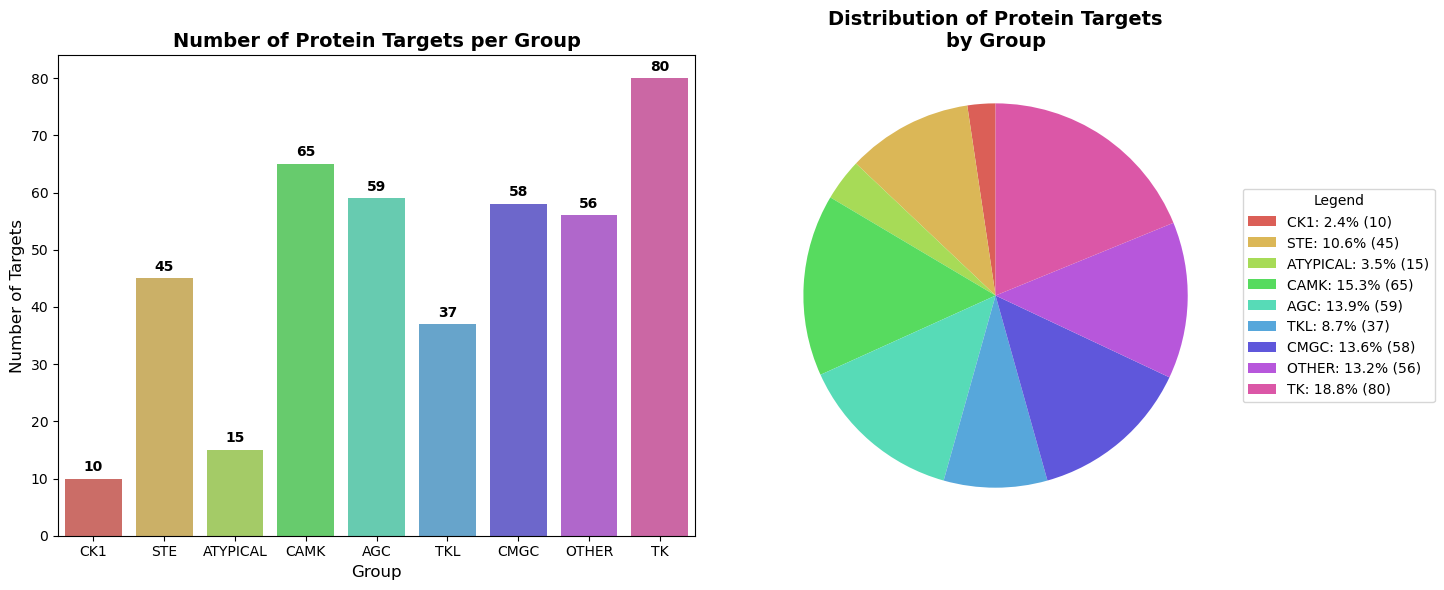
\includegraphics[width=0.49\textwidth]{../figures/ntarget_by_group.png}
    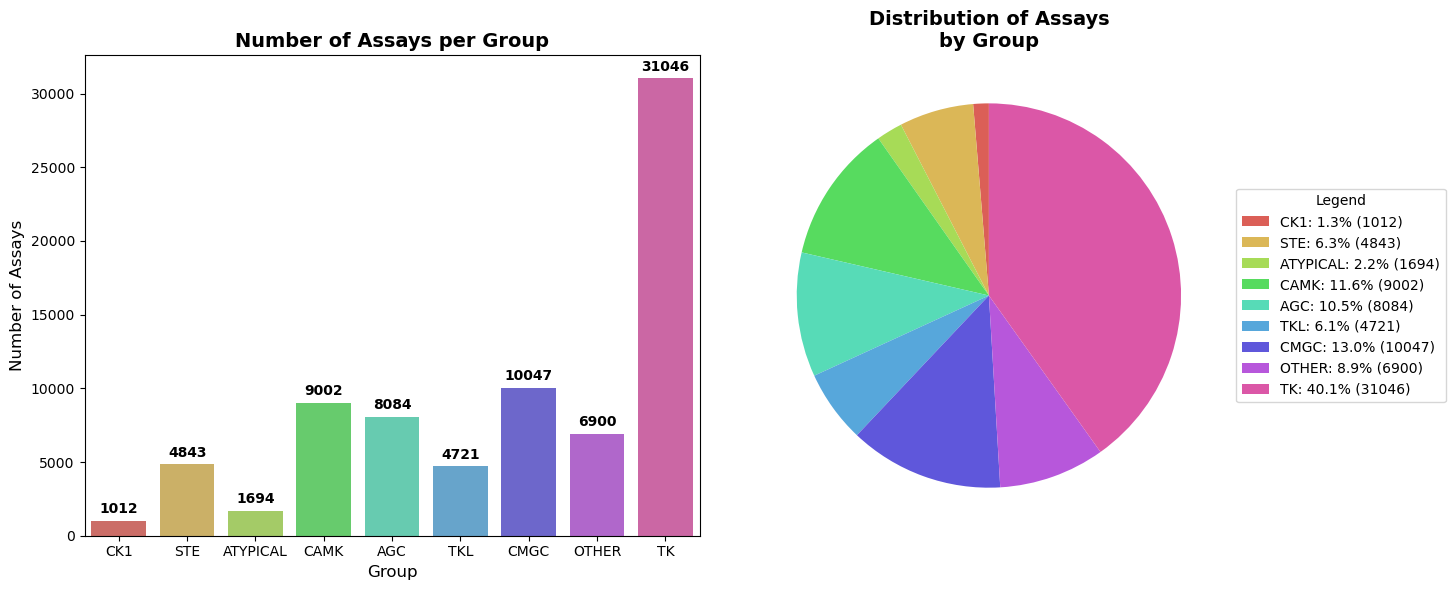
\includegraphics[width=0.49\textwidth]{../figures/nassay_by_group.png}
    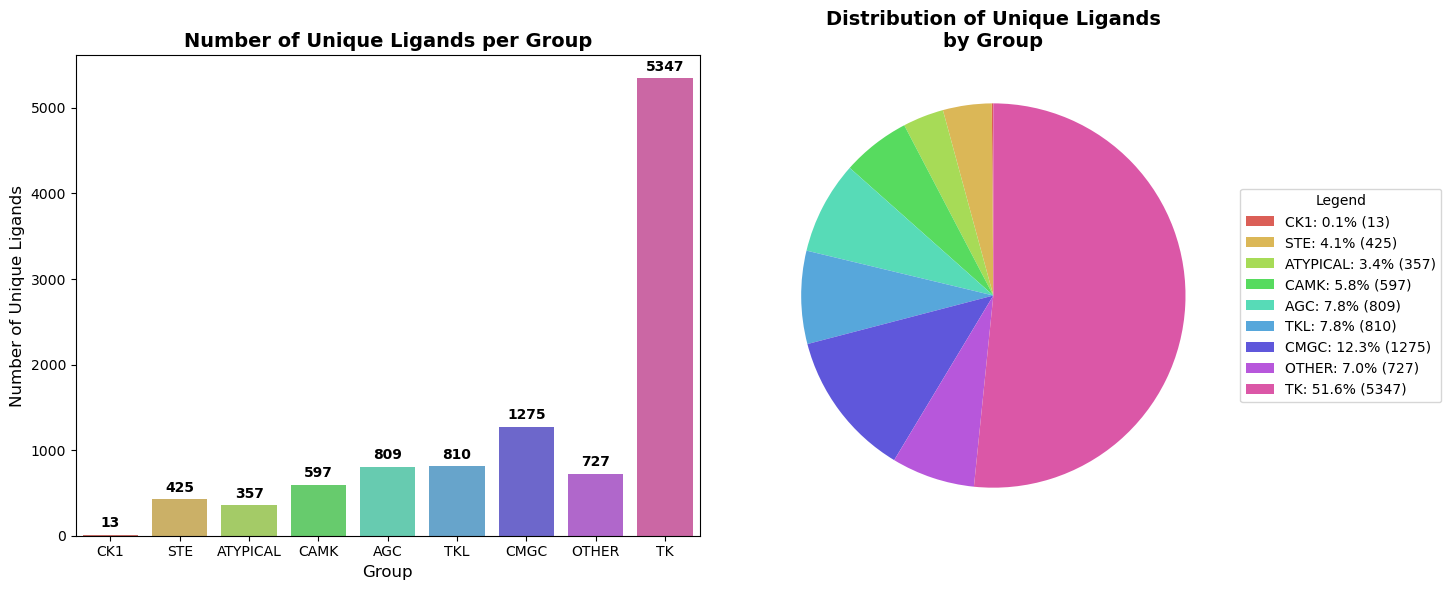
\includegraphics[width=0.49\textwidth]{../figures/nligand_by_group.png}
    \caption{Number of unique protein targets (top left), assays (top right), and ligands (bottom) belonging to each protein kinase group in the dataset.}
    \label{fig:group_atl_counts}
\end{figure}

After determining the set of ligands and their group relationships, Morgan fingerprints were computed using RDKit. 
Tanimoto similarity coefficients were then computed between these 2D fingerprints. 
These generated similarity values were clustered together using the ligand-group relationships described above and to generate the results described in the next section.
\section{Results}
To directly answer the main research question of this study (are ligands which are active within a particular protein kinase group more similar to one another than protein kinase ligands generally?), one can directly compare the distribution of similarity values computed with respect to all $9,995$ ligands in the dataset to the distribution of similarity values computed with respect to the ligands of individual protein kinase groups. 
These results are shown in Section~\ref{subsec:dist_results}. 
In addition, results show that there is (on average) a relationship between similarity threshold and enrichment with respect to both intra-group activity as well as assay activity (Section~\ref{subsec:results_enrichment}). 
However, as will be detailed in Section~\ref{sec:discussion}, there are several limitations to this study that must be accounted for before accepting any of the results presented below.
 
\subsection{Distribution}\label{subsec:dist_results}
Figure~\ref{fig:violin_plot} provides distributions for the ${N\choose 2}$ similarity values per group ($N$ = number of ligands), as well as the ${9,995 \choose 2} = 49,945,015$ similarity values calcualted for all kinase ligands in the dataset, with Table~\ref{tab:dist_stats} providing tthe statistics of each of distribution. 
\begin{figure}[H]
    \centering
    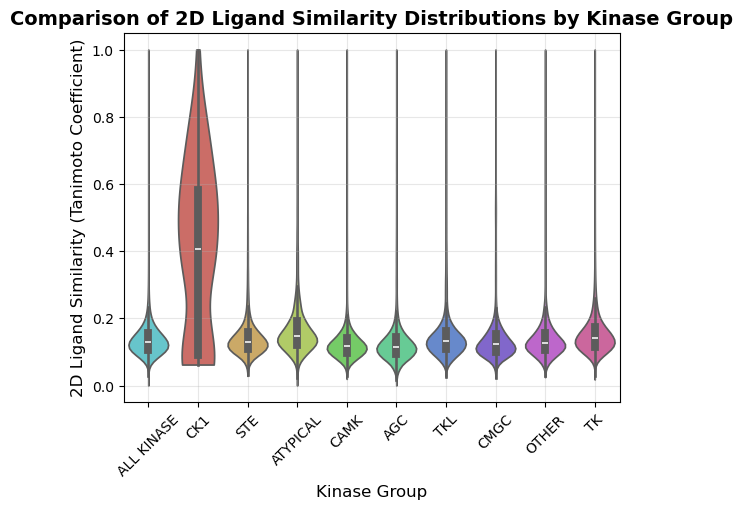
\includegraphics[width=0.75\textwidth]{../figures/violin_plot.png}
    \caption{Comparison of 2D structural similarity distributions by kinase group. Due to computational limitations a maximum of 1,000,000 (randomly selected) similarity values are shown for each distribution (note this only impact the ``ALL KINASE'' and ``TK'' distributions). When performing statistical analyses the entire set of similarity values was always used.}
    \label{fig:violin_plot}
\end{figure}

\begin{table}[!ht]
\centering
\resizebox{\textwidth}{!}{
\begin{tabular}{|l|l|l|l|l|l|l|}
    \hline
    \textbf{Distribution} & \textbf{N. Similarity Values} & \textbf{Mean} & \textbf{Median} & \textbf{Variance} & \textbf{Skewness} & \textbf{Kurtosis}\\ \hline
    ALL KINASE & 49,945,015 & 0.136 & 0.129 & 0.003 & 3.384 & 26.476 \\ \hline
    CK1 & 78 & 0.407 & 0.407 & 0.064 & 0.055 & -1.016 \\ \hline
    STE & 90,100 & 0.152 & 0.131 & 0.009 & 4.041 & 20.209 \\ \hline
    ATYPICAL & 63,546 & 0.180 & 0.149 & 0.014 & 3.095 & 11.453 \\ \hline
    CAMK & 177,906 & 0.133 & 0.117 & 0.006 & 4.895 & 29.897 \\ \hline
    AGC & 326,836 & 0.135 & 0.116 & 0.009 & 4.158 & 21.775 \\ \hline
    TKL & 327,645 & 0.153 & 0.133 &  0.009 & 3.693 & 17.759 \\ \hline
    CMGC & 812,175 & 0.144 & 0.122 & 0.009 & 3.829 & 17.676 \\ \hline
    OTHER & 263,901 & 0.144 & 0.127 & 0.007 & 4.441 & 25.778 \\ \hline
    TK & 14,292,531 & 0.153 & 0.140 & 0.004 & 3.176 & 18.678 \\ \hline
\end{tabular}}
\caption{Statistics for the distributions of ligand similarity values shown in Figure~\ref{fig:violin_plot}. Note that the number of similarity values belonging to each distribution will be equal to the number of pairs of ligands, i.e. ${N\choose 2}$.}\label{tab:dist_stats}
\end{table}

As can be seen from both Figure~\ref{fig:violin_plot} and Table~\ref{tab:dist_stats}, with the exception of the CK1 group there is not a clear difference between the similarity of ligands active within a single protein kinase group compared to the similarity of all protein kinase ligands. 
To measure the statistical significance of these findings, a Mann-Whitney U test (MWUT)~\cite{mann_whitney_1947} was performed with respect to each of the group distributions (note that since we have a total of 9 ``groups'' we are performing 9 different tests). 
The MWUT was chosen as an appropriate statistical test because of the following considerations:
\begin{enumerate}
    \item It is a non-parametric test (note that the distributions are not clearly normal, exponential, etc).
    \item The MWUT tests whether two samples have the same underlying distribution. Thus the test is more informative than just comparing a single statistic such as the mean or median. 
\end{enumerate}
The test was performed using the implementation provided by SciPy~\cite{scipy_2020,scipy_manual_2025}. 
If we let $X_G$ be the distribution of similarity values computed with respect to all ligands active within a given protein kinase group $G$ (CK1, STE, etc), and $Y$ be the distribution of similarity values computed with respect to all other protein kinase ligands in the dataset\footnote{Note that this definition of $Y$ is not the same as the ``ALL KINASE'' distribution shown above, and is necessary to ensure that $X_G$ and $Y$ are independent.}, then the test has the following null and alternative hypotheses~\cite{scipy_manual_2025}:\\
\begin{adjustwidth}{2.5em}{0pt}
$H_0$: The distribution underlying $X_G$ is not stochastically greater than the distribution underlying $Y$.\\\\
$H_a$: The distribution underlying $X_G$ is stochastically greater than the distribution underlying $Y$.\\
\end{adjustwidth}
\noindent
The test reports both a p-value and a U statistic. Since we're running multiple tests on different distributions, a Bonferonni correction is applied to all p-values to account for the multiple comparisons problem. 
The U statistic is considered the maximum value of $U1$ and $U2$ below:
\begin{equation}
U_1 = n_1n_2 + \frac{n_1(n_1+1)}{2}- R_1 \;\;\;\;\;\;\;\;\; U_2 = n_1n_2 + \frac{n_2(n_2+1)}{2}- R_2 \\
\end{equation}
Where $n_1$ and $n_2$ are the number of observations (i.e., similarity values) in $X_G$ and $Y$ respectively, and $R_1$ and $R_2$ are the sums of the ranks in $X_G$ and $Y$ after ranking all values such that the smallest value obtains rank 1 and the largest rank $n_1 + n_2$. 

The results from performing the MWUT are shown in Table~\ref{tab:mann_whitney_u}. 
As can be seen from the p-values in the table, according to the MWUT there is reason to reject the null hypothesis ($H_0$) stated above for several of the protein kinase groups. 
However, except for the CK1 group, the effect size is not very large (the extreme p-values are a result of the very large magnitude of $n_1$ and $n_2$). 
In the case of the CK1 group, both a large effect size (e.g., the difference of medians) and significant p-value ($3.10 \times 10^{-11}$) were observed. 
However, it should be noted that the number of ligands within the CK1 group is only 13, which in the wider context of chemistry + biology is unlikely to be a representative sample of all molecules which bind to CK1 proteins. 
There are also additional limitations of this study, such as the fact that not all proteins are equally well-represented in the dataset, that prevents these results from being definitive. 
These limitations will be discussed in more detail in Section~\ref{sec:discussion}. 
\begin{table}[!ht]
\centering
\footnotesize
\resizebox{\textwidth}{!}{
\def\arraystretch{1.2}
\begin{tabular}{|l|l|l|l|l|l|l|l|}
    \hline
\textbf{Group} & \textbf{Group size ($n_1$)} & \textbf{Comparison size ($n_2$)} & \textbf{Group Median} & \textbf{Comparison Median} & \textbf{$U_1$} & \textbf{$U_2$} & \textbf{p-value} \\ \hline
CK1 & 78 & 49,815,171 & 0.407 & 0.129 & $1.4002 \times 10^{13}$ & $1.6873 \times 10^{13}$ & $3.10 \times 10^{-11}$ \\ \hline
STE & 90,1000 & 45,787,665 & 0.131 & 0.129 & $2.1731 \times 10^{12}$ & $1.9524 \times 10^{12}$ & $2.48 \times 10^{-169}$ \\ \hline
ATYPICAL & 63,546 & 46,440,703 & 0.149 & 0.129 & $1.8801 \times 10^{12}$ & $1.0710 \times 10^{12}$ & $< 5 \times 10^{-324}$ \\ \hline
CAMK & 17,7906 & 44,156,503 & 0.117 & 0.130 & $3.1847 \times 10^{12}$ & $4.6710 \times 10^{12}$ & $1.0$ \\ \hline
AGC & 32,6836 & 42,186,705 & 0.116 & 0.131 & $5.4708 \times 10^{12}$ & $8.3173 \times 10^{12}$ & $1.0$ \\ \hline
TKL & 327,645 & 42,177,520 & 0.133 & 0.129 & $7.3358 \times 10^{12}$ & $6.4834 \times 10^{12}$ & $< 5 \times 10^{-324}$ \\ \hline
CMGC & 81,2175 & 38,014,840 & 0.122 & 0.130 & $1.4002 \times 10^{13}$ & $1.6873 \times 10^{13}$ & $1.0$ \\ \hline
OTHER & 26,3901 & 42,943,278 & 0.127 & 0.129 & $5.5731 \times 10^{12}$ & $5.7596 \times 10^{12}$ & $1.0$ \\ \hline
TK & 14,292,531 & 10,799,628 & 0.140 & 0.121 & $9.9533 \times 10^{13}$ & $5.4821 \times 10^{13}$ & $< 5 \times 10^{-324}$ \\ \hline
\end{tabular}}
\caption{Comparison of similarity distributions computed with respect to ligands active within particular protein kinase groups ($X_G$) vs the similarity distribution computed with respect to all other ligands in the dataset ($Y$). Shown p-values are calculated (with Bonferroni correction) from a Mann-Whitney U test (MWUT) where the alternative hypothesis is that the similarity values within the group are stochastically greater than the distribution of all similarity values. Note that although the MWUT is \textit{not} a test which considers the difference of medians, the median values are reported here to provide the reader with a more intuitive/familiar metric than the U statistic.}\label{tab:mann_whitney_u}
\end{table}

\subsection{Enrichment}\label{subsec:results_enrichment}
In addition to looking at the overall distribution of similarity values, the enrichment factor per group was also investigated.
Enrichment is defined here as how much more likely it is (on average) that two ligands are active within the same group $G$ given that their similarity is higher than some threshold.  
Prior research has looked at versions of this question before, and has found that when molecules are highly similar (Tanimoto similarity $\geq \; 0.85$) there is a $20-30\%$ chance they have similar biological activity~\cite{martin_kofron_traphagen_2002, chen_greenside_paik_sirota_hadley_butte_2015}. 
These probabilities are higher than random chance, but certainly leave room for exceptions. 
In the context of this work ``enrichment'' is defined according to equation~\ref{eq:enrichment}:
\begin{equation}\label{eq:enrichment}
    \footnotesize
    \frac{P(\text{two ligands active within group G} \; | \; \text{similarity} > \text{threshold})}{P(\text{two ligands active within group G})}
\end{equation}
\noindent

The motivation behind looking at enrichment is that, while there may not be a significant difference in the overall distributions of similarity values, one may still observe a higher-than-chance probability that two \textit{highly similar} ligands are active in the same group, and thus there may be a relationship between ligand similarity and intra-group activity at a sufficient threshold.  


Figure~\ref{fig:enrichment_plot} shows the enrichment values observed for different protein kinase groups. As is seen from the figure, there is generally a positive correlation between similarity threshold and the enrichment factor. 
However, there are good reasons to be skeptical of these results. 
It is unexpected for there to be a strong relationship between similarity and enrichment within either the ``Atypical'' or ``Other'' group, since the proteins within these groups are not related to one another in a meaningful way. 
Additionally, no relationship was observed for the TK group, even though these proteins are related in a meaningful way (they almost exclusively phosphorylate tyrosine residues). 
These counter-intuitive results are likely due to an imperfect definition of enrichment being used, as well as the general study limitations described in Section~\ref{sec:discussion}.

\begin{figure}[H]
    \centering
    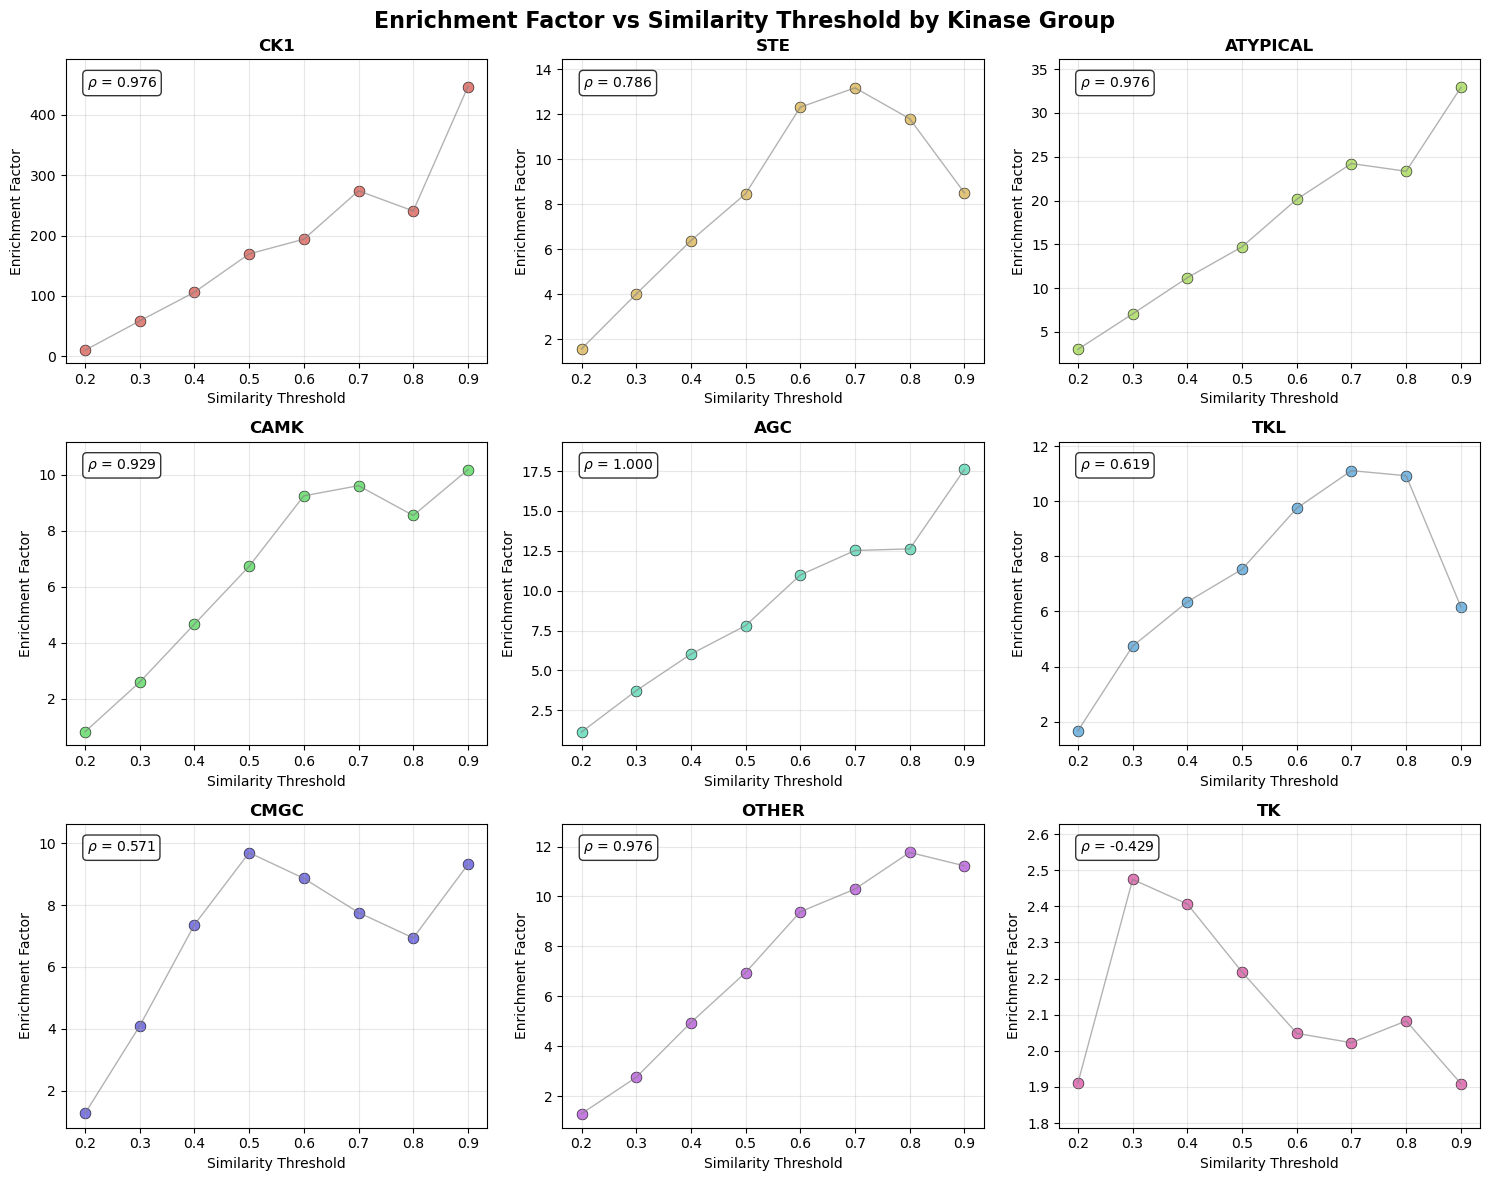
\includegraphics[width=0.75\textwidth]{../figures/enrichment_factor_by_group.png}
    \caption{Plot of tanimoto similarity threshold (x-axis) vs enrichment (y-axis) by protein kinase group.}
    \label{fig:enrichment_plot}
\end{figure}

The first issue with the definition of enrichment given above is that the magnitude of the enrichment factor depends upon the baseline probability of $P(\text{two ligands active within group G})$. 
While it intuitevly makes sense to normalize the conditional probability by the baseline when looking at enrichment, in practice this results in the enrichment factor being inflated when the baseline probability is extremely low.  
If one compares the baselines shown in Figure~\ref{fig:baseline_probs} to the observed enrichment values in Figure~\ref{fig:enrichment_plot}, they will see that there is a correlation between the baseline probability and observed enrichment values. 

\begin{figure}[H]
    \centering
    \includegraphics[width=0.75\textwidth]{../figures/baseline_prob_by_group.png}
    \caption{Baseline probability $P(\text{two ligands active within group G})$ for each protein kinase group. Note that the probabilities here will not sum to 1 because the sum of these baselines merely represents the probabilty that two randomly chosen ligands are both active within the same group.}
    \label{fig:baseline_probs}
\end{figure}

Another limitation is that the enrichment definition above does not account for ligands being active against the same target or within the same assay. 
Thus, the enrichment factor could be high for a given group simply because highly similar ligands are more likely to be active against the same target or within the same assay, but not necessarily because they are more likely to be active against other proteins in the same group. 
Figure~\ref{fig:enrichment_by_assay} shows that, while there is a significant spread in enrichment factor between individual assays, on average the enrichment factor exceeds $100$ when the similarity threshold is greater than $0.5$, and is close to $1000$ when the similarity threshold is greater than $0.8$. 
Since the per-assay enrichment factor is so enormous (on average), it must be taken into account when considering the results above. 

\begin{figure}[H]
    \centering
    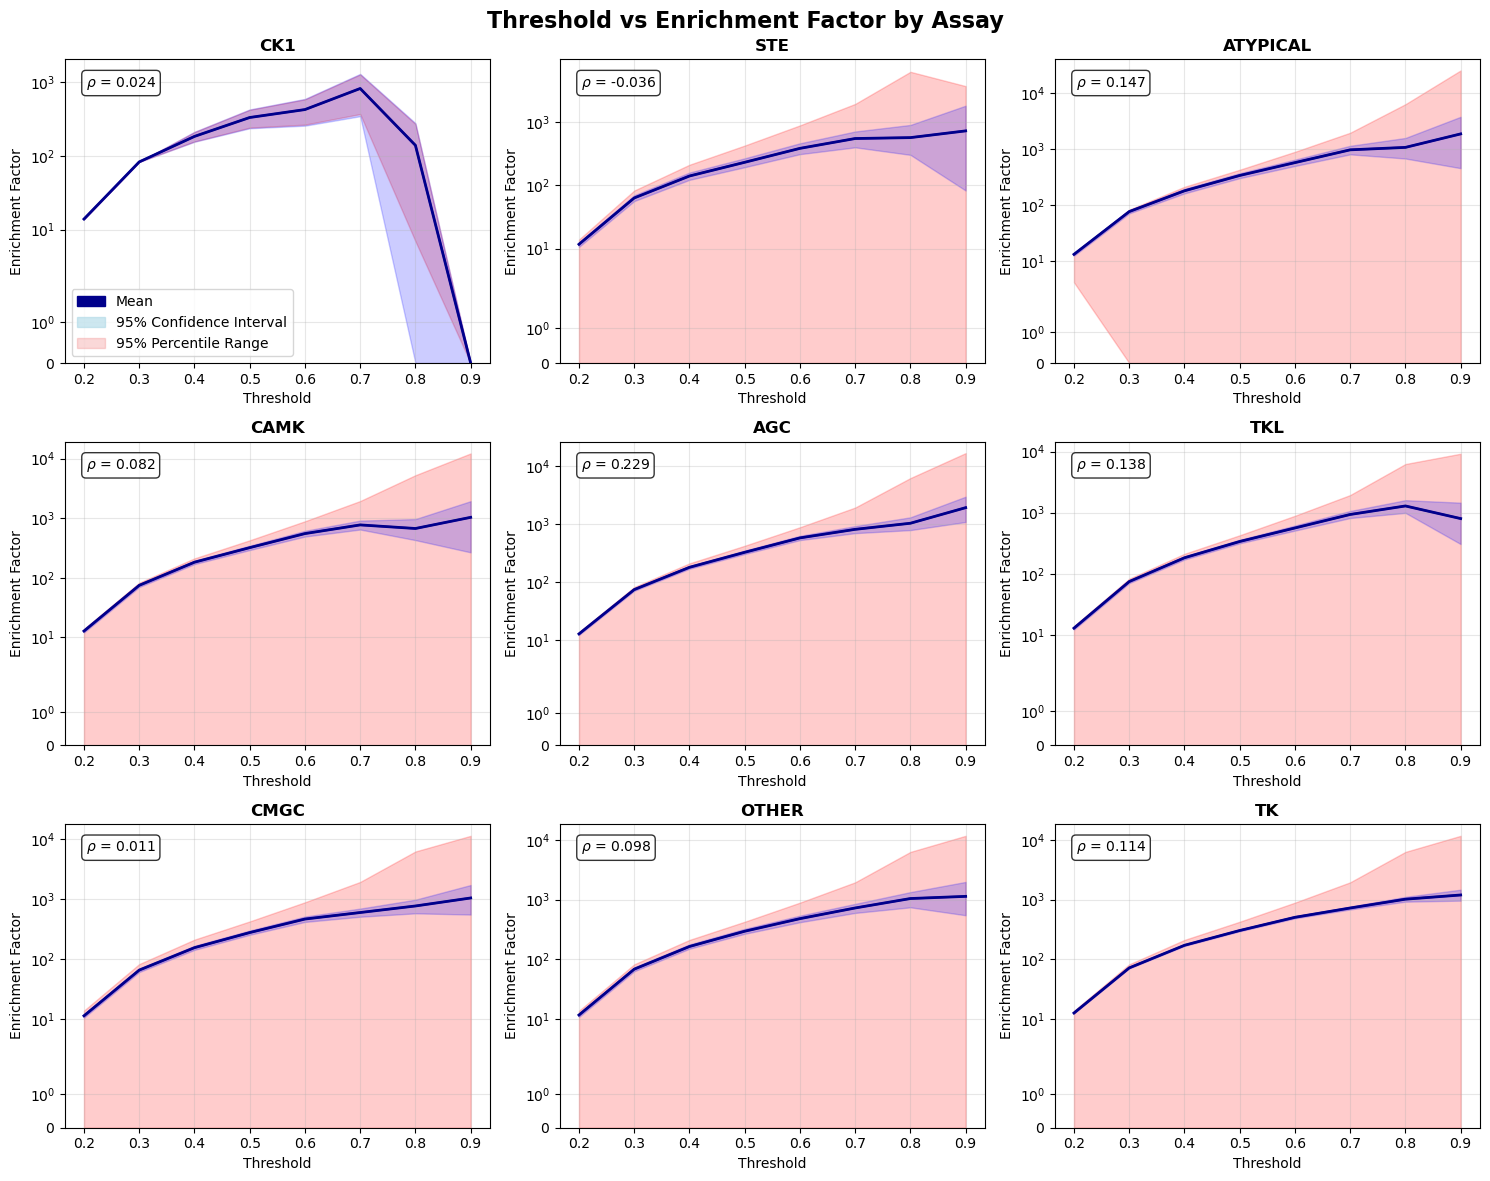
\includegraphics[width=0.75\textwidth]{../figures/enrichment_factor_by_assay.png}
    \caption{Plot of tanimoto similarity threshold (x-axis) and enrichment factor (y-axis) by assay. Here only assays which had at least 2 active ligands were considered. Assays were clustered based on the group membership of targets. It is worth noting that the enrichment factor is equal to $0$ when none of the active ligands in the assay have a similarity value greater than the threshold, which is why such a large percentile range is observed in each plot. It is also why there is a notable drop in the mean enrichment factor at a threshold of $0.8$ for CK1 assays.}\label{fig:enrichment_by_assay}
\end{figure}

\section{Discussion}\label{sec:discussion}
% include limitations here
% note that one limitation in definition of both enrichment and (perhaps) distribution analysis is that there is the confounder of same assay similarity
\begin{itemize}
    \item Not all protein targets are equally well-studied (see Figure~\ref{fig:assay_vs_ligand_plot})
    \item Only considered Morgan fingerprints + Tanimoto coefficients when measuring ``similarity'' of ligands
    \item Methodology does not directly account for differences in assay conditions, or the fact that even single proteins can have multiple binding sites
    \item Data gathered from ChEMBL may not reflect global trends
\end{itemize}

\begin{figure}[H]
    \centering
    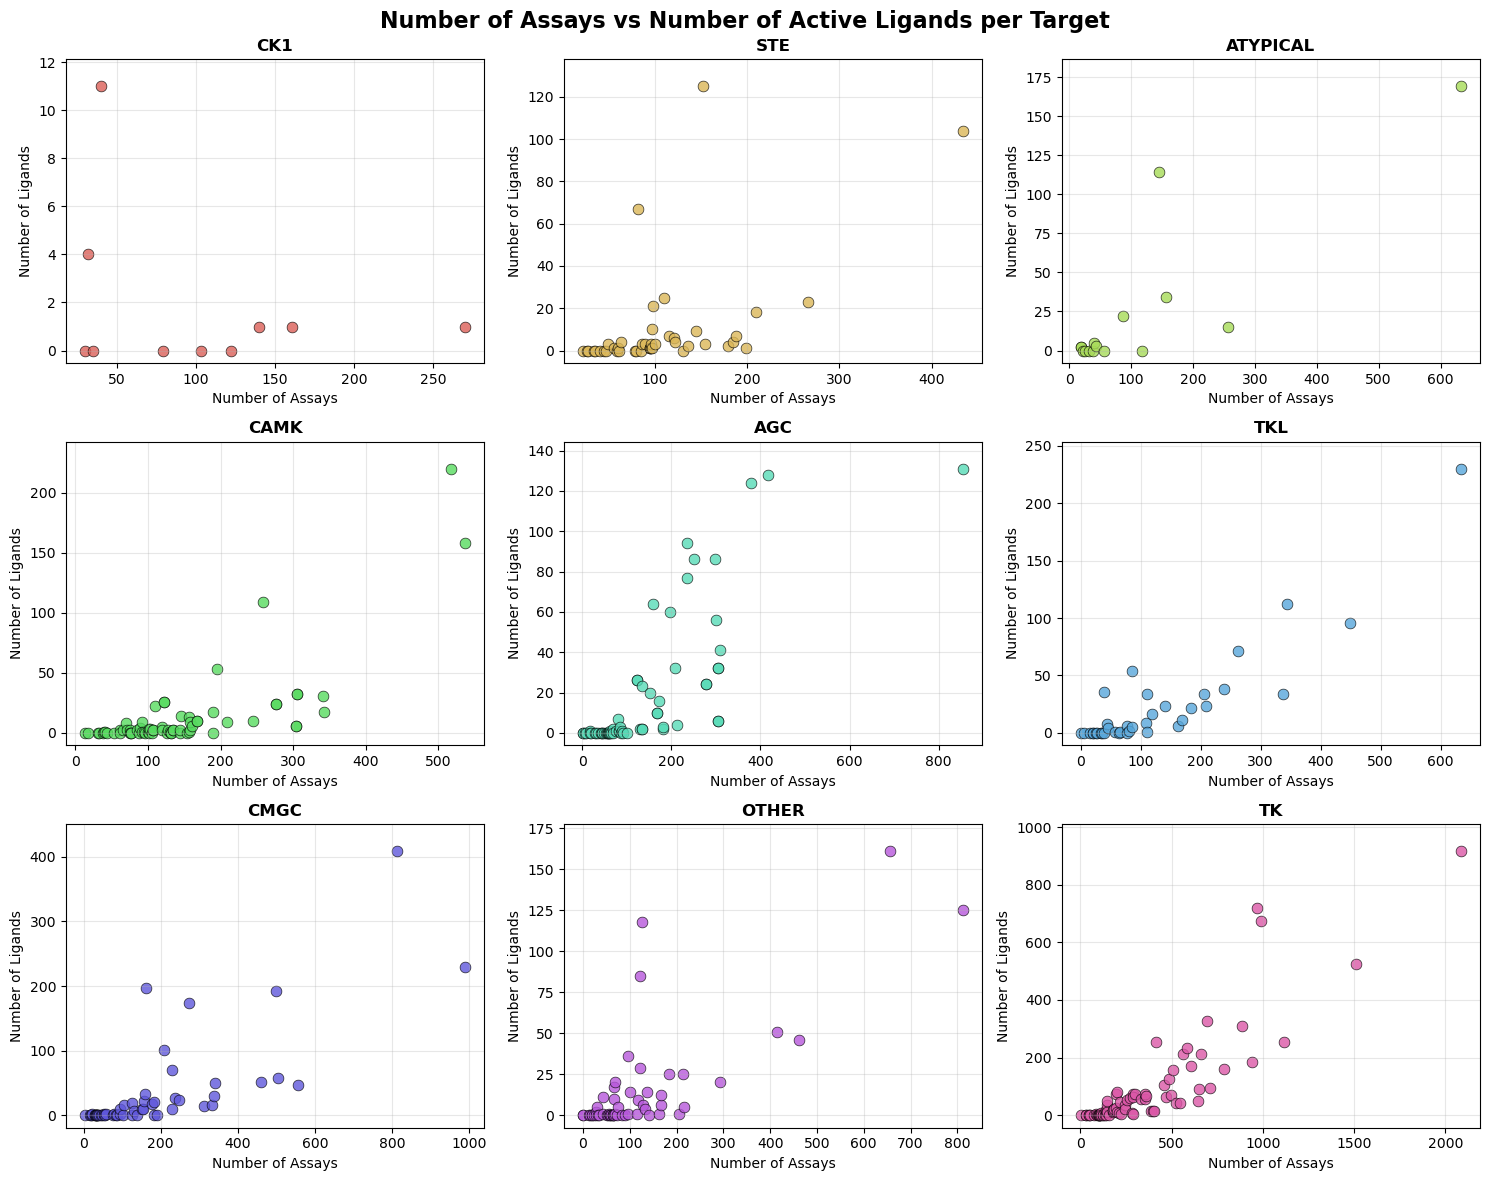
\includegraphics[width=0.85\textwidth]{../figures/assay_vs_ligand.png}
    \caption{Scatter plots showing the number of assays (x-axis) and ligands (y-axis) for each protein belonging to each protein kinase group.}
    \label{fig:assay_vs_ligand_plot}
\end{figure}

\section{Conclusion}
Overall, this study found no clear relationship between 2D ligand similarity and protein kinase group activity. Although significant differences were observed for the CK1 group, given the limitations outlined above further study is necessary before accepting these results. 

\section{Acknowledgements}
Much thanks to my advisor Dr.~Vincent Metzger for his guidance and input over the course of this project. I'd also like to thank Dr.~Jeremy Yang, Dr.~Cristian Bologa, and Dr.~Praveen Kumar for their feedback during weekly meetings over the course of the internship. Finally, I'd like to thank the   authors of ChEMBL DB~\cite{chembl_db_2023}.

\bibliographystyle{plain}\bibliography{report}

\end{document}
